%%%%%%%%%%%%%%%%%%%%%%%%%%EJERCICIO 10 %%%%%%%%%%%%%%%%%%%%%%%%%%%
\textbf{Ejemplo 10}\\
Resolver el problema anterior, suponiendo que el gradiente es escalonado con pagos semestrales.\\		

\textbf{Solución 10}\\
% La tabla irá centrada
\begin{center}
	\renewcommand{\arraystretch}{1.5}% Márgenes de las celdas
	% Creación de la cuadrícula de 2 columnas
	\begin{longtable}[H]{|c|c|}
		% Creamos una línea horizontal
		\hline
		% Definimos el color de la primera fila
		\rowcolor[HTML]{FFB183}
		\hline
		%%%%% INICIO ASIGNACIÓN PERÍODO FOCAL %%%%%%%
		%%%%%%%%%% INICIO TÍTULO
		% Lo que se hace aquí es mezclar las 2 columnas en una sola
		\multicolumn{2}{|c|}{\cellcolor[HTML]{FFB183}\textbf{1. Asignación período focal}} \\ \hline
		%%%%%%%%%% FIN TÍTULO
		%%%%% INICIO DECLARACIÓN DE VARIABLES %%%%%%%
		\multicolumn{2}{|c|}{$pf : 0 \; \textit{psv}$} \\ \hline
		%%%%%%%%%% INICIO TÍTULO
		% Lo que se hace aquí es mezclar las 2 columnas en una sola
		\multicolumn{2}{|c|}{\cellcolor[HTML]{FFB183}\textbf{2. Declaración de variables}} \\ \hline
		%%%%%%%%%% FIN TÍTULO
		%%%%%%%%%% INICIO DE MATEMÁTICAS
		\cellcolor[HTML]{FFB183}\textbf{Valores monetarios} & 
		\cellcolor[HTML]{FFB183}\textbf{Valores no monetarios} \\ \hline
		$VP = 500{.}000 \; \text{COP}$ & $n_{1} = 1 \; \textit{psv}$ \\ 
		$ $ & $n_{2} = 2 \; \textit{psv}$ \\ 
		$ $ & $n_{3} = 3 \; \textit{psv}$ \\ 
		$ $ & $n_{5} = 5 \; \textit{psv}$ \\ 
		$ $ & $n_{6} = 6 \; \textit{psv}$ \\ 
		$ $ & $i = 11{,}3552\% \; \textit{psv}$ \\ \hline
		%%%%%%%%%% FIN DE MATEMÁTICAS
		%%%%% FIN DECLARACIÓN DE VARIABLES

		\rowcolor[HTML]{FFB183}
		\hline
		\multicolumn{2}{|c|}{\cellcolor[HTML]{FFB183}\textbf{3. Diagrama de flujo de caja}} \\ \hline
		\multicolumn{2}{|c|}{ 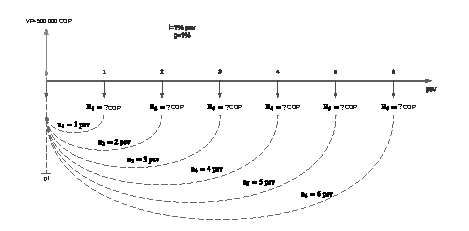
\includegraphics[trim=-78 -5 -78 -5]{7_Capitulo/img/ejemplos/10/10_1.pdf} } \\ \hline
		%%%%% INICIO FLUJO DE CAJA
		\rowcolor[HTML]{FFB183}
		\hline
		\multicolumn{2}{|c|}{\cellcolor[HTML]{FFB183}\textbf{4. Declaración de fórmulas}} \\ \hline
		%%%%%%%%%%%%% FIN INSERCIÓN DE IMAGEN
		%%%%% FIN FLUJO DE CAJA

		\multicolumn{2}{|c|}{ $(1+i_1)^{m_1} = (1+i_2)^{m_2} $ Equivalencia de tasas } \\  
		\multicolumn{2}{|c|}{ $VF = R\frac{(1+i)^{n} -1 }{i} $ Valor presente serie uniforme } \\ \hline
		
		%%%%%% INICIO DESARROLLO MATEMÁTICO
		\rowcolor[HTML]{FFB183}
		\hline
		%%%%%%%%%% INICIO TÍTULO
		\multicolumn{2}{|c|}{\cellcolor[HTML]{FFB183}\textbf{5. Desarrollo matemático}} \\ \hline
		%%%%%%%%%% FIN TÍTULO
		%%%%%%%%%% INICIO MATEMÁTICAS
		\multicolumn{2}{|c|}{ $(1+ 0{.}24)^{1} = (1+i)^{2}$ } \\ 
		\multicolumn{2}{|c|}{ $i = 11{,}3552\% \; \textit{psv}$ } \\ \hline

		%%%%%%%%%% FIN MATEMÁTICAS
		%%%%%% FIN DESARROLLO MATEMÁTICO
		%%%%%% INICIO RESPUESTA
		\rowcolor[HTML]{FFB183}
		\hline
		%%%%%%%%%% INICIO TÍTULO
		\multicolumn{2}{|c|}{\cellcolor[HTML]{FFB183}\textbf{6. Respuesta}} \\ \hline
		%%%%%%%%%% FIN TÍTULO
		%%%%%%%%%% INICIO RESPUESTA MATEMÁTICA
		\multicolumn{2}{|c|}{ 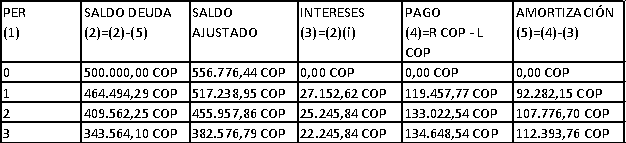
\includegraphics[trim=-78 -5 -78 -5]{7_Capitulo/img/ejemplos/10/10_2.pdf} } \\ \hline
	\end{longtable}
	% Se crean dos líneas en blanco para que no quede el siguiente texto tan pegado
	%\newline \newline % USARLO SI CREES QUE ES NECESARIO
\end{center}
%%%%%%%%%%%%%%%%%%%%%%%%%%FIN EJERCICIO 10 %%%%%%%%%%%%%%%%%%%%%%%%%%%
